\documentclass[aspectratio=169]{beamer}

% Theme and Color Setup
\usetheme{Madrid}
\usecolortheme{beaver} % Red/Gray theme, good for attention
\usepackage{tikz}
\usepackage{booktabs}
\usepackage{array}

% TikZ Library for graphing
\usetikzlibrary{calc, intersections}

% Title Information
\title{Unit 6: Imperfect Competition}
\subtitle{Monopolistic Competition and Oligopoly}
\author{Doğukan Günkördü}
\date{}

\begin{document}

%---------------------------------------------------------
% Title Slide
%---------------------------------------------------------
\begin{frame}
    \titlepage
\end{frame}

%---------------------------------------------------------
% Outline
%---------------------------------------------------------
\begin{frame}{Learning Objectives}
    In this chapter, we cover the "middle ground" of market structures:
    \begin{itemize}
        \item \textbf{Monopolistic Competition}:
            \begin{itemize}
                \item Product differentiation and non-price competition.
                \item Short-run profit/loss vs. Long-run equilibrium.
                \item Excess capacity and inefficiency.
            \end{itemize}
        \item \textbf{Oligopoly}:
            \begin{itemize}
                \item Interdependence and strategic behavior.
                \item Barriers to entry and Collusion.
                \item Game Theory (Dominant Strategies \& Nash Equilibrium).
            \end{itemize}
    \end{itemize}
\end{frame}

%=========================================================
% SECTION 1: MONOPOLISTIC COMPETITION
%=========================================================
\section{Monopolistic Competition}

\begin{frame}{Monopolistic Competition: Characteristics}
    Firms have characteristics of both Monopoly and Perfect Competition.
    \vspace{0.3cm}
    \begin{enumerate}
        \item<1-> \textbf{Many Sellers \& Easy Entry/Exit}: 
        \begin{itemize}
            \item Like perfect competition, there are many firms.
            \item Low barriers to entry allow firms to enter if there is profit.
        \end{itemize}
        \item<2-> \textbf{Differentiated Products}:
        \begin{itemize}
            \item Firms sell products that are \textit{similar} but not \textit{identical} (e.g., Fast Food: McDonald's vs. Wendy's).
            \item Gives the firm \textbf{some} control over price (Price Makers).
        \end{itemize}
        \item<3-> \textbf{Non-Price Competition}:
        \begin{itemize}
            \item Heavy use of advertising and branding to increase demand.
        \end{itemize}
        \item<4-> \textbf{Demand Curve}:
        \begin{itemize}
            \item Downward sloping, but very elastic due to many substitutes.
            \item $MR < Demand$.
        \end{itemize}
    \end{enumerate}
\end{frame}

%---------------------------------------------------------
% Short Run Graph (TikZ)
%---------------------------------------------------------
\begin{frame}{Short Run: Earning Economic Profit}
    \begin{columns}
        \column{0.5\textwidth}
        \textbf{Short Run Dynamics:}
        \begin{itemize}
            \item Profit Maximization Rule: Produce where $MR = MC$.
            \item Price ($P_m$) is pulled from the Demand curve.
            \item If $P > ATC$, the firm earns \textbf{Economic Profit}.
        \end{itemize}
        
        \column{0.5\textwidth}
        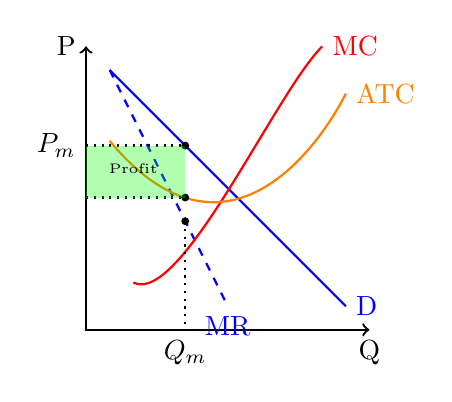
\begin{tikzpicture}[scale=0.6]
            \draw[thick, <->] (0,6) node[left]{P} -- (0,0) -- (6,0) node[below]{Q};
            % Demand and MR
            \draw[thick, blue] (0.5, 5.5) -- (5.5, 0.5) node[right]{D};
            \draw[thick, blue, dashed] (0.5, 5.5) -- (3, 0.5) node[below]{MR};
            % MC and ATC
            \draw[thick, red] (1, 1) .. controls (2, 0.5) and (4, 5) .. (5, 6) node[right]{MC};
            \draw[thick, orange] (0.5, 4) .. controls (3, 1) and (5, 4) .. (5.5, 5) node[right]{ATC};
            
            % Intersection MR=MC
            \filldraw (2.1, 2.3) circle (2pt); 
            \draw[dotted, thick] (2.1, 2.3) -- (2.1, 0) node[below]{$Q_m$};
            
            % Price on Demand Curve
            \filldraw (2.1, 3.9) circle (2pt);
            \draw[dotted, thick] (0, 3.9) node[left]{$P_m$} -- (2.1, 3.9);
            
            % ATC point
            \filldraw (2.1, 2.8) circle (2pt);
            \draw[dotted, thick] (0, 2.8) -- (2.1, 2.8);
            
            % Profit Box
            \fill[green, opacity=0.3] (0, 2.8) rectangle (2.1, 3.9);
            \node at (1, 3.4) {\tiny Profit};
        \end{tikzpicture}
    \end{columns}
\end{frame}

%---------------------------------------------------------
% Long Run Adjustment
%---------------------------------------------------------
\begin{frame}{Transition to the Long Run}
    What happens if firms earn profits in the short run?
    \vspace{0.5cm}
    \begin{itemize}
        \item<1-> \textbf{Entry}: New firms enter the market because entry is easy.
        \item<2-> \textbf{Impact on Existing Firms}: 
            \begin{itemize}
                \item More substitutes become available.
                \item \textbf{Demand shifts to the LEFT} for the existing firm.
                \item Demand becomes more elastic.
            \end{itemize}
        \item<3-> \textbf{Result}: Firms enter until Economic Profit = 0.
        \item<4-> \textit{Note: If firms were losing money, firms would exit, Demand would shift right.}
    \end{itemize}
\end{frame}

%---------------------------------------------------------
% Long Run Graph (TikZ)
%---------------------------------------------------------
\begin{frame}{Long Run Equilibrium}
    \begin{columns}
        \column{0.5\textwidth}
        \textbf{Long Run Outcomes:}
        \begin{itemize}
            \item $P = ATC$ (Zero Economic Profit).
            \item The Demand curve is tangent to the ATC curve.
            \item \textbf{Not Efficient}:
            \begin{itemize}
                \item $P > MC$ (Allocative Inefficiency).
                \item $P > \min ATC$ (Productive Inefficiency).
            \end{itemize}
        \end{itemize}
        
        \column{0.5\textwidth}
        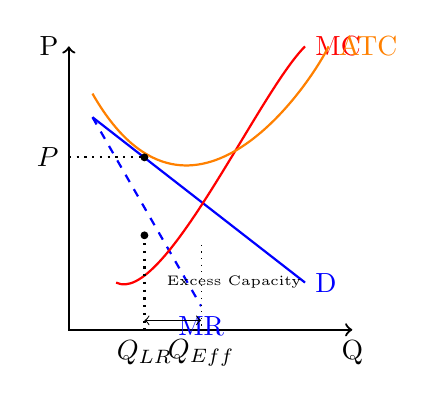
\begin{tikzpicture}[scale=0.6]
            \draw[thick, <->] (0,6) node[left]{P} -- (0,0) -- (6,0) node[below]{Q};
            % Demand and MR (Shifted Left)
            \draw[thick, blue] (0.5, 4.5) -- (5, 1) node[right]{D};
            \draw[thick, blue, dashed] (0.5, 4.5) -- (2.8, 0.5) node[below]{MR};
            % MC and ATC
            \draw[thick, red] (1, 1) .. controls (2, 0.5) and (4, 5) .. (5, 6) node[right]{MC};
            \draw[thick, orange] (0.5, 5) .. controls (2.5, 1.5) and (5, 5) .. (5.5, 6) node[right]{ATC};
            
            % Intersection MR=MC
            \filldraw (1.6, 2.0) circle (2pt); 
            \draw[dotted, thick] (1.6, 2.0) -- (1.6, 0) node[below]{$Q_{LR}$};
            
            % Tangency Point (P = ATC)
            \filldraw (1.6, 3.65) circle (2pt);
            \draw[dotted, thick] (0, 3.65) node[left]{$P$} -- (1.6, 3.65);
            
            % Min ATC
            \draw[dotted] (2.8, 1.8) -- (2.8, 0) node[below]{$Q_{Eff}$};
            \node at (3.5, 1) {\tiny Excess Capacity};
            \draw[<->] (1.6, 0.2) -- (2.8, 0.2);
        \end{tikzpicture}
    \end{columns}
\end{frame}

%---------------------------------------------------------
% Excess Capacity
%---------------------------------------------------------
\begin{frame}{Inefficiency and Excess Capacity}
    \begin{block}{Excess Capacity}
        The difference between the firm's actual output ($Q_{LR}$) and the productively efficient output (min ATC).
    \end{block}
    
    \begin{itemize}
        \item \textbf{Productive Efficiency}: Producing at minimum ATC.
        \item Monopolistic competitors produce on the \textit{downward slope} of ATC.
        \item \textbf{Real World Example}: 
        \begin{itemize}
            \item Gas stations on every corner. They have the capacity to serve more cars, but they don't have the demand.
            \item They are "underutilized."
        \end{itemize}
    \end{itemize}
\end{frame}

%=========================================================
% SECTION 2: OLIGOPOLY
%=========================================================
\section{Oligopoly}

\begin{frame}{Oligopoly: Characteristics}
    An industry dominated by a \textbf{few large firms}.
    \vspace{0.3cm}
    \begin{enumerate}
        \item \textbf{Few Sellers}: Top few firms control a large percentage of market share (e.g., Cell phones, Airlines, Soft Drinks).
        \item \textbf{High Barriers to Entry}: Hard for new firms to compete (high capital costs, patents).
        \item \textbf{Interdependence}:
        \begin{itemize}
            \item \alert{Key Concept}: One firm's actions \textbf{directly affect} the profits of another.
            \item Unlike Perfect Competition, you must watch your rival.
        \end{itemize}
        \item \textbf{Strategic Pricing}:
        \begin{itemize}
            \item \textbf{Collusion/Cartels}: Firms may agree to fix prices (illegal in US).
            \item \textbf{Price Leadership}: Dominant firm sets price, others follow.
        \end{itemize}
    \end{enumerate}
\end{frame}

%=========================================================
% SECTION 3: GAME THEORY
%=========================================================
\section{Game Theory}

\begin{frame}{Modeling Oligopoly: Game Theory}
    Because firms are interdependent, we use \textbf{Game Theory} to analyze strategy.
    
    \begin{itemize}
        \item \textbf{Players}: The firms (e.g., Firm A and Firm B).
        \item \textbf{Strategies}: Choices available (e.g., Price High vs. Price Low).
        \item \textbf{Payoff Matrix}: A table showing potential profits for every combination of choices.
    \end{itemize}
    
    \begin{block}{Dominant Strategy}
        A strategy that is the best choice for a player, \textbf{regardless} of what the other player chooses.
    \end{block}
\end{frame}

%---------------------------------------------------------
% Payoff Matrix Example
%---------------------------------------------------------
\begin{frame}{Analyzing a Payoff Matrix}
    \begin{center}
    \renewcommand{\arraystretch}{1.5}
    \begin{tabular}{cc|c|c|}
      & \multicolumn{1}{c}{} & \multicolumn{2}{c}{\textbf{Firm B}} \\
      & \multicolumn{1}{c}{} & \multicolumn{1}{c}{High Price} & \multicolumn{1}{c}{Low Price} \\\cline{3-4}
      \textbf{Firm A} & High Price & \underline{\$25}, \circled{\$25} & \underline{\$0}, \circled{\$35} \\\cline{3-4}
                      & Low Price & \underline{\$40}, \circled{\$5} & \underline{\$10}, \circled{\$10} \\\cline{3-4}
    \end{tabular}
    \end{center}
    
    \small
    \textbf{Finding Firm A's Strategy (Underlined):}
    \begin{itemize}
        \item If B goes High: A chooses Low (\$40 > \$25).
        \item If B goes Low: A chooses Low (\$10 > \$0).
        \item \textbf{Firm A's Dominant Strategy}: \alert{Low Price}.
    \end{itemize}
    
    \textbf{Finding Firm B's Strategy (Circled):}
    \begin{itemize}
        \item If A goes High: B chooses Low (\$35 > \$25).
        \item If A goes Low: B chooses Low (\$10 > \$5).
        \item \textbf{Firm B's Dominant Strategy}: \alert{Low Price}.
    \end{itemize}
\end{frame}

%---------------------------------------------------------
% Nash Equilibrium
%---------------------------------------------------------
\begin{frame}{Nash Equilibrium \& Prisoner's Dilemma}
    \begin{center}
    \textbf{Nash Equilibrium}: The outcome where neither player has an incentive to switch strategies given the other player's choice.
    \end{center}

    In the previous matrix:
    \begin{itemize}
        \item Both firms choose \textbf{Low Price}.
        \item Outcome: Both earn \$10.
    \end{itemize}
    
    \begin{alertblock}{The Prisoner's Dilemma}
        Notice that if both firms cooperated and priced \textbf{High}, they would both earn \$25.
        \begin{itemize}
            \item However, because of the incentive to cheat (Dominant Strategy), they end up in a worse outcome (\$10 each).
            \item This explains why \textbf{Cartels} are unstable; there is always an incentive to cheat.
        \end{itemize}
    \end{alertblock}
\end{frame}

%---------------------------------------------------------
% Advanced Game Theory (No Dominant Strategy)
%---------------------------------------------------------
\begin{frame}{What if there is NO Dominant Strategy?}
    Sometimes, a firm's best move depends on the other.
    
    \begin{columns}
        \column{0.5\textwidth}
        \begin{center}
        \renewcommand{\arraystretch}{1.5}
        \scriptsize
        \begin{tabular}{cc|c|c|}
          & \multicolumn{1}{c}{} & \multicolumn{2}{c}{\textbf{Red's}} \\
          & \multicolumn{1}{c}{} & \multicolumn{1}{c}{High} & \multicolumn{1}{c}{Low} \\\cline{3-4}
          \textbf{Grant's} & High & \underline{50}, 45 & \underline{25}, 35 \\\cline{3-4}
                           & Low & \underline{40}, 10 & \underline{15}, 20 \\\cline{3-4}
        \end{tabular}
        \end{center}
        \column{0.5\textwidth}
        \begin{itemize}
            \item \textbf{Grant}: High (50) $>$ Low (40). High (25) $>$ Low (15). \\ Grant has a Dominant Strategy: \textbf{High}.
            \item \textbf{Red}: If Grant High $\to$ High (45). If Grant Low $\to$ Low (20). \\ Red has \textbf{NO} Dominant Strategy.
        \end{itemize}
    \end{columns}
    \vspace{0.5cm}
    \textbf{Result}: Red knows Grant will play High. Therefore, Red plays High to get 45. 
    \\ \textbf{Nash Equilibrium}: High / High.
\end{frame}

%=========================================================
% SECTION 4: SUMMARY
%=========================================================
\section{Summary}

\begin{frame}{Comparison of Market Structures}
    \begin{table}
    \centering
    \resizebox{\textwidth}{!}{
    \begin{tabular}{|l|c|c|}
    \hline
    \rowcolor{gray!30}
    \textbf{Feature} & \textbf{Monopolistic Competition} & \textbf{Oligopoly} \\ \hline
    \textbf{Number of Firms} & Many & Few (Dominant) \\ \hline
    \textbf{Barriers to Entry} & Low / Easy Entry & High Barriers \\ \hline
    \textbf{Product} & Differentiated & Identical or Differentiated \\ \hline
    \textbf{Control over Price} & Some (Brand loyalty) & Significant (Interdependence) \\ \hline
    \textbf{Long Run Profit} & Zero (Normal Profit) & Positive Economic Profit \\ \hline
    \textbf{Efficiency} & Inefficient ($P>MC$) & Inefficient ($P>MC$) \\ \hline
    \end{tabular}
    }
    \end{table}
\end{frame}

\begin{frame}{Final Review Tips}
    \begin{enumerate}
        \item \textbf{Graphing Monopolistic Comp}:
        \begin{itemize}
            \item Always draw Demand and MR separate (MR below D).
            \item In Long Run, ATC is tangent to D (price), not MR.
            \item Remember: Excess Capacity is the gap between current Q and min ATC output.
        \end{itemize}
        \item \textbf{Game Theory}:
        \begin{itemize}
            \item Circle/Underline payoffs to avoid confusion.
            \item A "Dominant Strategy" implies the same choice regardless of the opponent.
            \item Nash Equilibrium: No regrets; no incentive to switch.
        \end{itemize}
    \end{enumerate}
\end{frame}

\end{document}
